\documentclass[11pt,a4paper,twocolumn]{article}

% === Core Packages ===
\usepackage[margin=2cm]{geometry}
\usepackage[utf8]{inputenc}
\usepackage[T1]{fontenc}
\usepackage{times}
\usepackage{amsmath,amssymb}
\usepackage{graphicx}
\usepackage{booktabs}
\usepackage{float}
\usepackage{enumitem}
\usepackage{tikz}
\usepackage{pgfplots}
\pgfplotsset{compat=1.18}
\usetikzlibrary{arrows.meta,shapes.geometric,positioning,calc,decorations.markings,fit,backgrounds}

% === Citation (IEEE style) ===
\usepackage[numbers,sort&compress]{natbib}
\bibliographystyle{IEEEtranN}

% === Hyperref ===
\usepackage[hidelinks]{hyperref}
\usepackage{xurl}

% === Settings ===
\setlength{\parindent}{1em}
\setlength{\parskip}{0.3em}

% === Title ===
\title{\textbf{Decentralizuotas reputacijos tinklas:\\Natūralaus visuomenės organizavimo sistema}}
\author{Pavel Kudrna\\Prague, Czechia\\Draft v1 --- March 2026}
\date{}

\begin{document}
\maketitle

% ============================================================
% ABSTRACT
% ============================================================
\begin{abstract}
Teisingumo jausmas---įsitikinimas, kad neteisybės ištaisomos, o nuopelnai atlyginami---yra stipriausia visuomenę vienijanti jėga. Kai centralizuotos valdymo institucijos negali suteikti šio jausmo, nes teisės įgyvendinimo kaina viršija pačios teisės vertę, socialinė sanglauda yra griaunama. Dabartinės institucinės struktūros nesugeba išspręsti reikšmingos ginčų dalies sistemiškai lygiai taip pat, kaip centrinis planavimas nesugeba paskirstyti išteklių: dėl informacijos asimetrijos, trūkstamų grįžtamojo ryšio kilpų ir sprendimų priėmėjų atsiribojimo nuo savo sprendimų padarinių. Šiame straipsnyje pristatomas reputacijos socialinis tinklas (RSN): decentralizuotas, nepaperkamas, cenzūrai atsparus komunikacijos sluoksnis, sukurtas remiantis decentralizuotais identifikatoriais (DID), leidžiantis pseudonimiškiems dalyviams skelbti, tikrinti ir vartoti reputacijos informaciją apie realaus pasaulio elgesį. Pagrindinis mechanizmas remiasi trimis projektavimo principais: (1)~asimetrine kaštų struktūra, kurioje reputacijos duomenų skaitymas yra pigus, o rašymas reikalauja patikrinamų pastangų; (2)~nedeterministiniu tikrintojų parinkimo protokolu, pagrįstu nuosekliuoju maišymu, kuris įkainoja radikalius teiginius per didėjančius iteracijų kaštus; ir (3)~rinkos vairuojamu reputacijos autoritetų modeliu, kuriame privatūs tikrintojai stato savo sukauptą reputaciją už jų patvirtinamų teiginių tikslumą. Gauta architektūra sukuria emergentinę meritokratiją be centrinio koordinavimo ir įgalina laipsnišką, grįžtamą migracijos kelią nuo esamų valstybės administruojamų sistemų.
\end{abstract}

% ============================================================
% 1. INTRODUCTION
% ============================================================
\section{Įvadas}

\subsection{Centralizuoto pasitikėjimo problema}

Šiuolaikinis valdymas remiasi esmine prielaida: kad centralizuotos institucijos gali tarpininkauti pasitikėjimą tarp nepažįstamų žmonių plačiu mastu. Teismai sprendžia ginčus. Registrai patvirtina nuosavybę. Reguliavimo institucijos užtikrina standartus. Šios institucijos buvo sukurtos epochoje, kai informacijos buvo stinga, komunikacija buvo lėta, o įgaliojimų perdavimas centrinei institucijai buvo vienintelis įmanomas koordinavimo mechanizmas. Tačiau centralizuotas valdymas žlunga dėl tų pačių struktūrinių priežasčių kaip ir centrinis planavimas: informacijos asimetrijos, trūkstamų grįžtamojo ryšio kilpų ir sprendimų priėmėjų atsiribojimo nuo savo sprendimų padarinių.

Ši prielaida žlunga, pavyzdžiui, kai institucinio tarpininkavimo kaina viršija ginčo vertę. Įsivaizduokite nuomininką, kuris atranda, kad jo išsinuomotas butas neturi teisiškai reikalaujamo elektros saugos sertifikato---sąlygos, kelianti tiesioginį pavojų gyvybei. Nuomininko teisinė teisė atsisakyti sutarties yra vienareikšmiška. Tačiau šios teisės įgyvendinimo per teismų sistemą kaina viršija užstato ir priteistinų nuostolių piniginę vertę, net įskaitant galimą įstatyminę kompensaciją~\cite{czcourtfees}. Racionalus atsakas yra susitaikyti su nuostoliu ir pasitraukti.

Tai nėra patologinis kraštutinis atvejis. Tai yra numatytoji patirtis reikšmingai ginčų klasei, kurioje žala yra reali, bet piniginis statymas nesiekia ribos, ties kuria institucinis įgyvendinimas tampa ekonomiškai racionalus. Rezultatas---sistema, kuri struktūriškai palankiai vertina blogus veikėjus: tie, kurie kenkia kitiems žemiau šios ribos, gali veikti nebaudžiami, nes teisingumo siekimo kaina tenka nukentėjusiai šaliai.

Aukščiau pateiktas pavyzdys paimtas iš autoriaus teisinės aplinkos---Čekijos civilinės teisės sistemos. Kitose teisinėse tradicijose---precedentu grįstoje bendrojoje teisėje, paprotinėje teisėje, mišriose sistemose---teisingumas žlunga skirtingais būdais ir skirtingu mastu, priklausomai nuo jurisdikcijos kultūrinių ir procedūrinių ypatumų. Skaitytojai tikriausiai atpažins lygiaverčius pavyzdžius iš savo aplinkos. Struktūriškai universalus yra šablonas: ginčai, kurių vertė nesiekia ekonomiškai racionalaus įgyvendinimo ribos, baigiasi nuostoliu, kurį prisiima nukentėjusi šalis. RSN nežada tobulo teisingumo---jis tik sumažina struktūrinį pranašumą, kurį blogi veikėjai turi, kai institucinis įgyvendinimas yra neekonomiškas.

\subsection{Kodėl esami sprendimai yra nepakankami}

\textbf{Decentralizuoto identiteto (DID) sistemos}~\cite{did2022} teikia kriptografinius mechanizmus savarankiškai valdomam tapatybės tvarkymui, bet daugiausia dėmesio skiria tapatybės tikrinimui, neatsakydamos į platesnį elgesio reputacijos klausimą.

\textbf{Sielai pririšti žetonai (SBT)}~\cite{weyl2022} užfiksuoja įžvalgą, kad reputacija yra neperduodama, bet remiasi blokų grandinės infrastruktūra su mastelio apribojimais ir neatsako į ekonomines paskatas, valdančias informacijos įvedimą. Susijusios koncepcijos, tokios kaip nuopelnų žetonai (pvz., Liberland), remiasi panašia filosofija, bet lieka susietos su konkrečiomis jurisdikcinėmis sistemomis.

\textbf{Decentralizuotos autonominės organizacijos (DAO)}~\cite{buterin2014} įgyvendina valdymą per išmaniąsias sutartis, bet atkartoja plutokratinę dinamiką, kai įtaka yra proporcinga kapitalui. Kvadratinis balsavimas~\cite{buterin2019} iš dalies tai sušvelnina, bet riboja praktinį pritaikymą. DAO taip pat susiduria su esmine \emph{orakulo problema}: išmaniosios sutartys negali patikimai patikrinti realaus pasaulio būsenų be patikimo išorinio šaltinio, o ši problema neturi bendro sprendimo blokų grandinės architektūroje.

Nė viena esama sistema neapjungia decentralizacijos, atsparumo cenzūrai, pseudonimiškumo, patikrinamos įėjimo kainos ir emergentinio konsensuso.

\subsection{Įnašai}

Šis straipsnis pateikia šiuos įnašus:
\begin{enumerate}[nosep]
\item \textbf{Reputacijos socialinio tinklo (RSN)} apibrėžimas---decentralizuoto protokolo, plečiančio DID sistemą, kad būtų palaikomas dvišalis reputacijos mainai.
\item \textbf{Nedeterministinis tikrintojų parinkimo protokolas}, pagrįstas nuosekliuoju maišymu~\cite{karger1997}.
\item \textbf{Brangaus radikalumo principas}, įkainojantis teiginius pagal jų atstumą nuo tinklo konsensuso per tris besidauginančius kaštų kanalus.
\item \textbf{Patikimo autoriteto modelis} su asimetrinėmis paskatomis, kai melagingas patvirtinimas kainuoja katastrofiškai daugiau nei teisėti mokesčiai.
\item \textbf{Laipsniškas migracijos kelias} per lygiagrečią fiskalinę infrastruktūrą.
\end{enumerate}

% ============================================================
% 2. DESIGN PRINCIPLES
% ============================================================
\section{Projektavimo principai}

RSN architektūrą riboja penki nediskutuotini projektavimo principai.

\textbf{Tęstinumas ir evoliucija.} Sistema sugyvena su esamomis institucijomis pereinamuoju neapibrėžtos trukmės laikotarpiu. Perėjimas turi būti grįžtamas kiekviename etape.

\textbf{Savanoriškumas ir atsakomybė.} Dalyvavimas yra savanoriškas, bet savanoriškumas siejamas su atsakomybe: dalyvis, prisiimantis institucinės funkcijos kontrolę, kartu prisiima ir lydinčias pareigas.

\textbf{Įvairovė ir kultūrinis neutralumas.} Konsensusas atsiranda iš dvišalių sąveikų, o ne iš iš anksto nustatytų taisyklių, primestų sistemos kūrėjų.

\textbf{Atsparumas ir atsparumas cenzūrai.} Tinklo cenzūravimo kaina turi viršyti jo toleravimo kainą. Tik visiškas totalitarizmas---pragaištingomis politinėmis ir ekonominėmis sąnaudomis---gali nuslopinti sistemą.

\textbf{Konsensusas ir įgyvendinimas.} Sistema įtraukia žmogiškuosius polinkius į smulkmeniškumą, pyktį ir keršto pasitenkinimą kaip laikančiąsias savybes. Netinkamas elgesys nėra draudžiamas; jis yra įkainojamas.

% ============================================================
% 3. SYSTEM OVERVIEW
% ============================================================
\section{Sistemos apžvalga}

\subsection{Reputacijos socialinis tinklas}

RSN yra decentralizuotas, tarpusavio (peer-to-peer) komunikacijos sluoksnis, kuriame dalyviai keičiasi patikrinama informacija apie realaus pasaulio elgesį. Jo apibrėžiančios savybės yra: decentralizuota ir necenzūruojama infrastruktūra; pseudonimiškas dalyvavimas per DID; asimetrinė kaštų struktūra (skaitymas pigus, rašymas brangus); kriptografinis patikrinamumas; ir \textbf{standartų palaikymas}---mašininiu būdu skaitomi formatai informacijai, sklindančiai per tinklą, autoritetų teikiamoms paslaugoms (teiginio sudarymas, patvirtinimas, liudytojo paslauga) ir politikos formatui, įskaitant taisykles, skirtas įvertinti sandorio šalies reputaciją ir politikos neatitikimo riziką (tarp deklaruoto ir faktinio elgesio).

\subsection{Architektūriniai komponentai}

RSN sudaro keturi pagrindiniai komponentai (\ref{fig:architecture} pav.):
\begin{enumerate}[nosep]
\item \textbf{DID sluoksnis.} Dalyvių tapatybės su deklaruotomis taisyklėmis, reputacijos metaduomenimis ir tinklo maršrutizavimu.
\item \textbf{Teiginių protokolas.} Struktūrizuotas formatas teiginiams apie realaus pasaulio įvykius skelbti.
\item \textbf{Tikrinimo tinklas.} Decentralizuotas protokolas tikrintojams priskirti, naudojant nuoseklųjį maišymą.
\item \textbf{Reputacijos apibendrinimo sluoksnis.} Paslaugos, kuriančios žmogaus skaitomas reputacijos santraukas.
\end{enumerate}

\begin{figure}[ht]
\centering
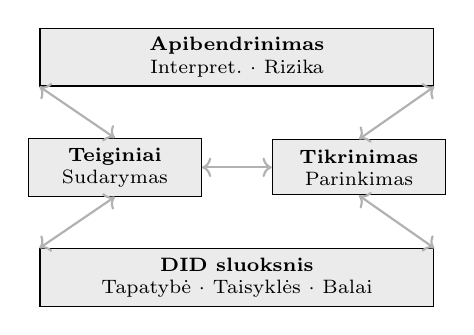
\begin{tikzpicture}[
    layer/.style={draw, minimum height=0.7cm, align=center, font=\scriptsize, fill=black!8},
    arr/.style={<->, thick, gray!60}
]
\node[layer, minimum width=5cm] (agg) at (0,2.8) {\textbf{Apibendrinimas}\\Interpret.\ $\cdot$ Rizika};
\node[layer, minimum width=2.2cm] (claim) at (-1.55,1.4) {\textbf{Teiginiai}\\Sudarymas};
\node[layer, minimum width=2.2cm] (verif) at (1.55,1.4) {\textbf{Tikrinimas}\\Parinkimas};
\node[layer, minimum width=5cm] (did) at (0,0) {\textbf{DID sluoksnis}\\Tapatybė $\cdot$ Taisyklės $\cdot$ Balai};

\draw[arr] (agg.south west) -- (claim.north);
\draw[arr] (agg.south east) -- (verif.north);
\draw[arr] (claim.east) -- (verif.west);
\draw[arr] (claim.south) -- (did.north west);
\draw[arr] (verif.south) -- (did.north east);
\end{tikzpicture}
\caption{RSN keturių sluoksnių architektūra.}
\label{fig:architecture}
\end{figure}

\subsection{Dalyvių vaidmenys}

Tikrinimo transakcijoje dalyvauja iki šešių skirtingų DID vaidmenų (\ref{fig:roles} pav.): \textbf{Išdavėjas} ($DID_I$, sukuria ir pateikia teiginį), \textbf{Subjektas} ($DID_S$, DID, apie kurį yra teiginys---gali sutapti su Išdavėju), \textbf{Autoritetas} ($DID_A$, patvirtina teiginį už mokestį; taip pat gali teikti liudytojo paslaugas---\emph{neprivaloma}), \textbf{Liudytojas} ($DID_{W_{1..n}}$, inkognito tikrintojo sąžiningumo stebėtojas per iššūkio kodus---\emph{neprivaloma}), \textbf{Tikrintojas} ($DID_V$, algoritmiškai parinktas teiginiui paskelbti) ir \textbf{RSN} (tinklas, kuriame skelbiami patikrinti teiginiai). Bet koks vaidmuo gali būti deleguotas kitam DID (7.4 skyrius). Autoritetas dažnai apjungia patvirtinimą su liudytojo paslaugomis, bet abi funkcijos yra logiškai nepriklausomos.

\begin{figure}[ht]
\centering
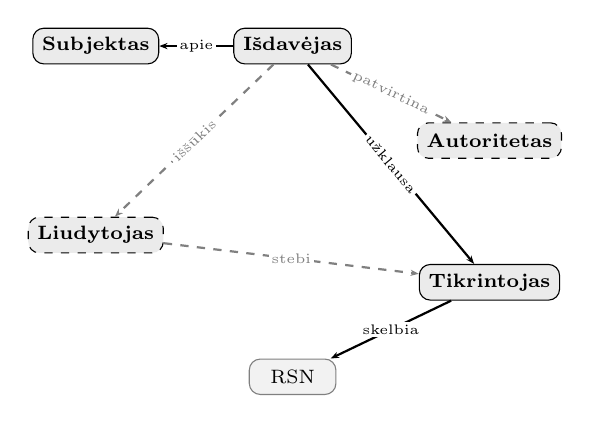
\begin{tikzpicture}[
    role/.style={draw, rounded corners, minimum width=1.1cm, minimum height=0.45cm, align=center, font=\scriptsize, fill=black!8},
    opt/.style={draw, rounded corners, minimum width=1.1cm, minimum height=0.45cm, align=center, font=\scriptsize, fill=black!8, dashed},
    arr/.style={-{Stealth[length=3pt]}, thick},
    oarr/.style={-{Stealth[length=3pt]}, thick, dashed, gray},
    lbl/.style={font=\tiny, fill=white, inner sep=1pt}
]
\node[role] (I) at (0,2.4) {\textbf{Išdavėjas}};
\node[role] (S) at (-2.5,2.4) {\textbf{Subjektas}};
\node[opt] (A) at (2.5,1.2) {\textbf{Autoritetas}};
\node[opt] (W) at (-2.5,0) {\textbf{Liudytojas}};
\node[role] (V) at (2.5,-0.6) {\textbf{Tikrintojas}};
\node[role, fill=black!5, draw=gray] (N) at (0,-1.8) {RSN};

\draw[arr] (I) -- node[lbl] {apie} (S);
\draw[oarr] (I) -- node[lbl,sloped] {patvirtina} (A);
\draw[oarr] (I) -- node[lbl,sloped] {iššūkis} (W);
\draw[arr] (I) -- node[lbl,sloped] {užklausa} (V);
\draw[oarr] (W) -- node[lbl] {stebi} (V);
\draw[arr] (V) -- node[lbl] {skelbia} (N);
\end{tikzpicture}
\caption{DID vaidmenys tikrinimo transakcijoje. Punktyras = neprivaloma (Autoritetas, Liudytojas).}
\label{fig:roles}
\end{figure}

\subsection{Nepaperkamumas: keturios jėgos}

RSN nepaperkamumas kyla ne iš vieno mechanizmo, o iš keturių vienalaikių jėgų. Nė viena nepakanka pati savaime; tik jų derinys daro korupcijos bandymą ekonomiškai neracionalų.

\textbf{Nenuspėjamas taikinys.} Kiekvieno teiginio tikrintojas parenkamas nedeterministiškai per nuoseklųjį maišymą (5.3 skyrius). Užpuolikas negali iš anksto nusitaikyti į konkretų tikrintoją papirkimui, nes tikrintojo tapatybė yra teiginio turinio ir ankstesnių iteracijų funkcija, o ne išdavėjo pasirinkimas.

\textbf{Reputacinis svertas---lėtai aukštyn, greitai žemyn.} Reputacija gali būti įgyjama tik palaipsniui, per nuolatinį nuoseklų elgesį. Tačiau ji gali būti katastrofiškai prarasta vieną kartą apgaulingai patvirtinus (6.2 skyrius). Ši asimetrija reiškia, kad metų metais sukaupta reputacija gali būti sugriauta vieno nesąžiningo patvirtinimo; optimali strategija lieka atmesti įtartinus teiginius.

\textbf{Viešas pažadas.} Kiekvienas DID turėtojas viešai deklaruoja savo politiką---mašininiu būdu skaitomą taisyklių rinkinį, kurio įsipareigoja laikytis. Deklaracijos ir faktinio elgesio neatitikimas yra aptinkamas ir įkainojamas kaip reputacinis nusižengimas, sunkesnis nei pats pažeidimas (7.3 skyrius). Todėl veidmainystė kainuoja daugiau nei tiesioginis nesąžiningumas.

\textbf{Tinklo atakos kaštų asimetrija.} Tinklo cenzūravimo ar destabilizavimo kaina auga netiesiškai su tinklo dydžiu ir tankiu, o jo toleravimo kaina lieka pastovi. Kad cenzūra atsipirktų, centralizuotas veikėjas turėtų ją taikyti visame tinkle---reikalaujant priemonių, neproporcingų bet kokiai įsivaizduojamai naudai (10 skyrius).

% ============================================================
% 4. DECENTRALIZED IDENTITY MODEL
% ============================================================
\section{Decentralizuoto identiteto modelis}

\subsection{DID su ypatingomis savybėmis}

RSN plečia W3C DID Core specifikaciją~\cite{did2022} šiais elementais: \textbf{Deklaruotos taisyklės} (mašininiu būdu skaitomi elgesio įsipareigojimai), \textbf{Reputacijos metaduomenys} (apibendrintas elgesio balas) ir \textbf{Tinklo maršrutizavimas} (kintantis onion šliuzas, atskirtas nuo stabilios pozicijos žiede).

\subsection{Teiginio gyvavimo ciklas}

Teiginys pereina šešis etapus (\ref{fig:lifecycle} pav.): sudarymas, neprivalomas autoriteto patvirtinimas, tikrintojo parinkimas per nuoseklųjį maišymą, tikrinimo sprendimas (priimti arba atmesti su iteracija), paskelbimas ir reputacijos atnaujinimas visoms šalims.

\begin{figure}[ht]
\centering
\begin{tikzpicture}[
    stp/.style={draw, rounded corners=2pt, minimum width=1.3cm, minimum height=0.45cm, align=center, font=\tiny, fill=black!5},
    arr/.style={-{Stealth[length=3pt]}, thick},
    lbl/.style={font=\tiny, fill=white, inner sep=1pt}
]
\node[stp] (comp) at (0,0) {Sudaryti\\teiginį};
\node[stp, dashed] (auth) at (2.0,0) {Autoritetas\\patvirtina};
\node[stp] (hash) at (4.0,0) {Maiša ir\\žiedo\\priskyrimas};
\node[stp] (ver) at (2.0,-1.6) {Tikrintojas\\tikrina};
\node[stp, double] (pub) at (0,-1.6) {Paskelbta};
\node[stp] (rej) at (4.0,-1.6) {Atmesta\\kaštai $\uparrow$};

\draw[arr] (comp) -- (auth);
\draw[arr] (auth) -- (hash);
\draw[arr] (hash) -- (ver);
\draw[arr] (ver) -- node[lbl] {\checkmark} (pub);
\draw[arr] (ver) -- node[lbl] {$\times$} (rej);
\draw[arr] (rej) -- ++(0,0.8) -| (hash);
\end{tikzpicture}
\caption{Teiginio gyvavimo ciklas su iteracijos kilpa.}
\label{fig:lifecycle}
\end{figure}

\subsection{Ryšys su W3C DID Core}

RSN tapatybės modelis yra tinkamas W3C DID Core specifikacijos~\cite{did2022} superrinkinys. Visi RSN DID yra galiojantys W3C DID. RSN specifiniai plėtiniai yra užkoduoti kaip DID dokumento savybės, apibrėžtos atskiroje DID metodo specifikacijoje, suderinamoje su esama infrastruktūra, tokia kaip ION~\cite{buchner2021} ir Ceramic~\cite{ceramic2023}.

% ============================================================
% 5. VERIFICATION AND PROPAGATION
% ============================================================
\section{Informacijos tikrinimas ir sklaida}

\subsection{Informacijos įvedimo kaina}

Pagrindinis RSN ekonominis principas yra asimetrija tarp skaitymo ir rašymo. Reputacijos duomenų skaitymas artėja prie nulinių ribinių kaštų dalyviams, kurie yra DID tinklo dalis ir turi jų reputaciją atitinkančią prieigą---naujokai turi palaipsniui užsitarnauti platesnę prieigą (žr. apsaugą nuo išnaudojimo). Rašymas---suprantamas kaip tvarus reputacijos materializavimas į tinklą, o ne kaip vienkartinis techninis veiksmas---reikalauja patikrinamų kaupiamųjų investicijų per tris dimensijas: \textbf{laiką} (gyvenimo metai, praleisti nuosekliai elgiantis, vykdant įsipareigojimus ir puoselėjant santykius), \textbf{energiją} (pastangos, investuotos į sąžiningą sandėrį, rūpestį partnerystėmis ir ilgalaikį patikimumą) ir \textbf{pinigus} (investicija į savo vardą---profesinis tobulėjimas, darbo kokybė, padarytos žalos atlyginimas). Reputacijos negalima nusipirkti akimirksniu---ji yra viso gyvenimo kaupimo rezultatas, kurį sistema tik padaro matomą ir perkeliamą tarp kontekstų. Vienkartiniai techniniai protokolo kaštai (kriptografiniai parašai, tikrintojų mokesčiai) yra nereikšmingi, palyginti su šia pamatine investicija.

\subsection{Socialinis grafas ir kontaktų gylis}

RSN iš esmės yra socialinis tinklas: kiekvienas DID prideda kontaktus (kitus DID), kurie leidžia ryšį. Šie kontaktai turi savo kontaktus ir taip toliau. Algoritminė tikrintojų paieška veikia konfigūruojamame susietų kontaktų gylyje $h$ (pvz., $h=3$: tiesioginiai kontaktai, jų kontaktai ir kontaktų kontaktai). Ši architektūra nereikalauja vienos globalios blokų grandinės---ji natūraliai skatina bendruomenių / grupių, turinčių persidengimų su kitomis bendruomenėmis, atsiradimą. Kiekvienas DID dalyvis privalo turėti paskelbtą \textbf{politiką}---mašininiu būdu skaitomą taisyklių rinkinį, valdantį, kaip vertinamos gaunamos užklausos. Politikos pažeidimai yra fiksuojami tinkle kaip neigiami artefaktai.

\subsection{Algoritminis tikrintojų parinkimas}

Tikrinimo protokolas naudoja nuoseklųjį maišymą~\cite{karger1997} (\ref{fig:verifier} pav.). Tikrinimas yra mokama paslauga: tikrintojai veikia už mokestį, sukurdami rinką, kurioje konkurencija lemia kainodarą, greitį ir patikimumą.

\textbf{1 žingsnis.} Teiginio dokumentas sujungiamas su ankstesnės iteracijos maišos rezultatu (arba $\varnothing$ pirmojoje iteracijoje) ir maišomas:
\begin{equation}
\text{poz} = f_h(\text{teiginys} \| \text{prev\_hash})
\label{eq:hash}
\end{equation}

Algoritmas turi įtraukti \emph{visą kelią} iš visų ankstesnių užklausų ir atsakymų---ne vien ankstesnės iteracijos maišą. Kiekvieno tikrintojo pilnas atsakymas (priėmimas, atmetimas, nurodyta kaina, priežastis) yra pridedamas prie augančio dokumento, patikrinamas per kriptografinius parašus kiekviename žingsnyje.

\textbf{2 žingsnis.} Maiša priskiriama $N$ pozicijoms nuosekliojo maišymo žiede, tolygiai paskirstytoms (pvz., $N=4$: $+0^{\circ}, +90^{\circ}, +180^{\circ}, +270^{\circ}$). Iš kiekvienos pozicijos pagal laikrodžio rodyklę atliekama paieška parenka artimiausią DID kaip tikrintojo kandidatą (\ref{fig:multipoint} pav.). $N$ yra kintamas parametras, galintis priklausyti nuo šiuo metu aktyvių DID procento, paros meto arba istorinio tinklo reagavimo.

\textbf{3 žingsnis.} Tikrintojas priima (paskelbia, statydamas reputaciją) arba atmeta (grįždamas į 1 žingsnį su atmetimo maiša). Kai mazgas neatsako, nepaisant to, kad deklaruoja aktyvią būseną, kita užklausa turi įtraukti visus atsakymus iš visų $N$ ankstesnių tikrintojų kandidatų.

\textbf{Apsauga nuo išnaudojimo.} Tiksliniai DID gali nustatyti mokesčius ar prieigos apribojimus užklausoms iš naujų DID su maža reputacija. Šis laipsniškas mechanizmas (ne dvejetainis) verčia naujokus kaupti reputaciją per tikrą veiklą, prieš laisvai vartojant kitų duomenis.

\begin{figure}[ht]
\centering
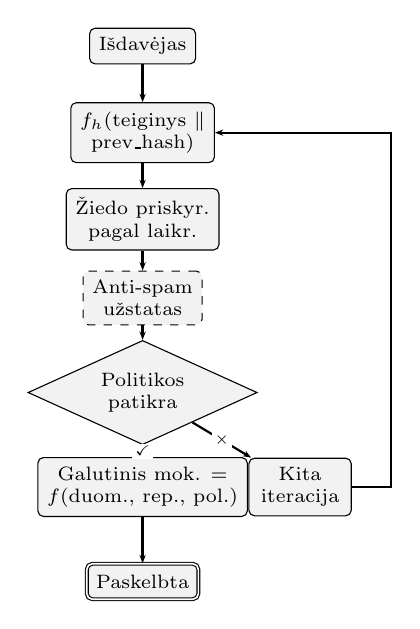
\begin{tikzpicture}[
    box/.style={draw, rounded corners=2pt, minimum width=1.3cm, minimum height=0.45cm, align=center, font=\scriptsize, fill=black!5},
    dec/.style={draw, diamond, aspect=2.2, minimum width=0.9cm, align=center, font=\scriptsize, fill=black!5},
    arr/.style={-{Stealth[length=3pt]}, thick},
    lbl/.style={font=\tiny, fill=white, inner sep=1pt}
]
\node[box] (iss) at (0,0) {Išdavėjas};
\node[box] (hash) at (0,-1.1) {$f_h$(teiginys $\|$\\prev\_hash)};
\node[box] (ring) at (0,-2.2) {Žiedo priskyr.\\pagal laikr.};
\node[box, dashed] (spam) at (0,-3.2) {Anti-spam\\užstatas};
\node[dec] (check) at (0,-4.4) {Politikos\\patikra};
\node[box] (rej) at (2,-5.6) {Kita\\iteracija};
\node[box] (fee) at (0,-5.6) {Galutinis mok. =\\$f$(duom., rep., pol.)};
\node[box, double] (pub) at (0,-6.8) {Paskelbta};

\draw[arr] (iss) -- (hash);
\draw[arr] (hash) -- (ring);
\draw[arr] (ring) -- (spam);
\draw[arr] (spam) -- (check);
\draw[arr] (check) -- node[lbl] {$\times$} (rej);
\draw[arr] (check) -- node[lbl] {\checkmark} (fee);
\draw[arr] (fee) -- (pub);
\draw[arr] (rej.east) -- ++(0.5,0) |- (hash.east);
\end{tikzpicture}
\caption{Tikrintojų parinkimo protokolas. Anti-spam užstatas yra neprivalomas ir gali būti grąžinamas. Galutinis mokestis mokamas tik priėmimo atveju.}
\label{fig:verifier}
\end{figure}

Kiekvienas atmetimas prideda pilną tikrintojo atsakymą (įskaitant priežastis ir sąlygas) prie teiginio dokumento, plėsdamas jo turinį. Iš išplėsto dokumento nedeterministiškai apskaičiuojama nauja maiša, priskiriama kitai žiedo pozicijai ir parenkanti kitą tikrintoją. Viso kelio dokumentavimas yra privalomas---išdavėjas negali numatyti ar paveikti kito tikrintojo. Jei tikrintojas ignoruoja užklausą, nepaisant suderinamos deklaruotos politikos, liudytojai (jei yra) tai fiksuoja, ir išdavėjas gali pridėti liudytojų įrodymus galutinio paskelbimo metu.

\begin{figure}[ht]
\centering
\begin{tikzpicture}[scale=0.65]
% Ring
\draw[thick] (0,0) circle (2.2cm);
% DID nodes on ring
\foreach \a in {10,55,80,120,150,195,230,260,305,340} {
  \fill[black!40] (\a:2.2) circle (1.5pt);
}
% Hash offset arrow pointing to initial position
\draw[-{Stealth[length=3pt]}, thick, black!60] (0,0) -- node[font=\tiny,above,sloped,pos=0.6] {$f_h$} (37:2.2);
\fill[black] (37:2.2) circle (2pt);
\node[font=\tiny,anchor=south west] at (37:2.35) {$h_0$};
% N=4 points offset from h0 by +0, +90, +180, +270
\foreach \offset/\l in {0/P1,90/P2,180/P3,270/P4} {
  \pgfmathsetmacro{\ang}{37+\offset}
  \node[fill=black, circle, inner sep=1.5pt] (p\offset) at (\ang:2.2) {};
  \node[font=\tiny,font=\bfseries] at (\ang:2.75) {\l};
  % clockwise search arc
  \draw[-{Stealth[length=2.5pt]}, thick, gray] (\ang:2.2) arc (\ang:\ang+30:2.2);
}
\node[font=\scriptsize, align=center] at (0,0) {Maišos\\žiedas};
\node[font=\tiny, align=center] at (0,-3.2) {$h_0 = f_h(\text{teiginys})$, tada $+0^{\circ},+90^{\circ},+180^{\circ},+270^{\circ}$\\Kiekvienas taškas $\rightarrow$ paieška pagal laikrodžio rodyklę};
\end{tikzpicture}
\caption{Kelių taškų parinkimas ($N{=}4$). Maiša $h_0$ nustato poslinkį; 4 taškai tolygiai paskirstyti nuo $h_0$.}
\label{fig:multipoint}
\end{figure}

\subsection{Liudytojų protokolas}

\textbf{Liudytojo} vaidmuo suteikia inkognito atskaitomybę už tikrintojo sąžiningumą per kriptografinį iššūkio kodų protokolą:

\textbf{W1 žingsnis.} Užklausėjas pasirašo tikrinimo užklausą ir siunčia ją $N_w$ liudytojams---kontaktams iš užklausėjo socialinio tinklo arba specializuotiems liudytojų paslaugų teikėjams, veikiantiems už mokestį.

\textbf{W2 žingsnis.} Kiekvienas liudytojas $w_i$ pasirašo visą pasirašytą užklausą, išsaugo originalų parašą $\sigma_i$ ir apskaičiuoja iššūkio kodą $c_i = h(\sigma_i)$. Iššūkio kodas pridedamas prie užklausos.

\textbf{W3 žingsnis.} Užklausa, dabar nešanti $N_w$ iššūkio kodų, siunčiama tikrintojui. Tikrintojas mato kodus, bet \emph{negali nustatyti}, kas yra liudytojai ar ar kodai atitinka tikrus parašus.

\textbf{W4 žingsnis (sąžiningas tikrintojas).} Jei tikrintojas atsako pagal savo deklaruotą politiką, iššūkio kodai lieka neperskaitomi. Liudytojai niekada neatskleidžiami. Jokie papildomi duomenys neskelbiami.

\textbf{W5 žingsnis (politikos pažeidimas).} Jei tikrintojas pažeidžia savo politiką (ignoruoja užklausą, atsako nenuosekliai), užklausėjas turi liudytojų originalius parašus $\sigma_i$. Šie gali būti paskelbti kaip lydintys duomenys: bet kas gali patikrinti $c_i = h(\sigma_i)$, įrodydamas, kad liudytojas buvo. Užklausėjas gali paskelbti savarankiškai---tikrintojas jau pasirašė iššūkio kodus savo atsakyme.

\textbf{Blefo savybė.} Užklausėjas gali pakeisti kai kuriuos ar visus iššūkio kodus atsitiktinėmis reikšmėmis. Tikrintojas negali atskirti tikrų kodų (paremtų aukštos reputacijos autoritetais) nuo triukšmo. Šis \emph{netikrumas} yra įgyvendinimo mechanizmas: kiekviena užklausa neša riziką, kad gerbiamas autoritetas stebi inkognito. Šio spaudimo palaikymo kaina yra beveik nulinė (atsitiktinių skaičių generavimas), o galima nesąžiningumo kaina tikrintojui yra katastrofiška. Sąžiningas elgesys yra skatinamas net nesant tikrų liudytojų.

\textbf{Autoritetas kaip liudytojas.} Autoritetas, patvirtinantis teiginį, gali apjungti liudytojo paslaugas: „Patvirtinu jūsų teiginį ir tarnauju kaip inkognito liudytojas tikrinimo metu.“ Tai natūralus verslo modelis---autoritetas jau turi kontekstą. Tačiau abu vaidmenys yra logiškai nepriklausomi.

\subsection{Brangaus radikalumo principas}

Trys kaštų kanalai vienu metu dauginasi (\ref{fig:radicalism} pav.):

\textbf{1 kanalas: iteracijos kaštai.} Kiekvienas atmetimas priverčia naują iteraciją, sunaudojančią laiką ir išteklius. Tiesinis augimas.

\textbf{2 kanalas: dokumento išpūtimas.} Kiekviena iteracija prideda pilną tikrintojo atsakymą prie teiginio dokumento. Augimas yra tiesinis, bet su baziniu poslinkiu: pradinis krovinys (teiginio turinys, autoriteto patvirtinimas, kriptografiniai parašai) jau turi netrivialų dydį $B_0$. Bendras dydis po $k$ iteracijų: $S(k) = B_0 + k \cdot \Delta$, kur $\Delta$ yra vidutinis atsakymo dydis.

\textbf{3 kanalas: tikrintojo rizikos priedas.} Rizika yra subjektyvi. Tikrintojas įvertina, ar užklausiančio DID deklaruotos politikos prieštarauja tikrintojo komerciniams, socialiniams ar politiniams interesams. Priedas gali eksponentiškai augti su suvokiamu atstumu nuo tikrintojo „idealo“: $P(d) = \alpha \cdot e^{\beta d}$, kur $d$ yra tikrintojo subjektyvi atstumo metrika. Peržengus asmeninę neperžengiamą ribą, tikrintojas gali visiškai atsisakyti.

\begin{figure}[ht]
\centering
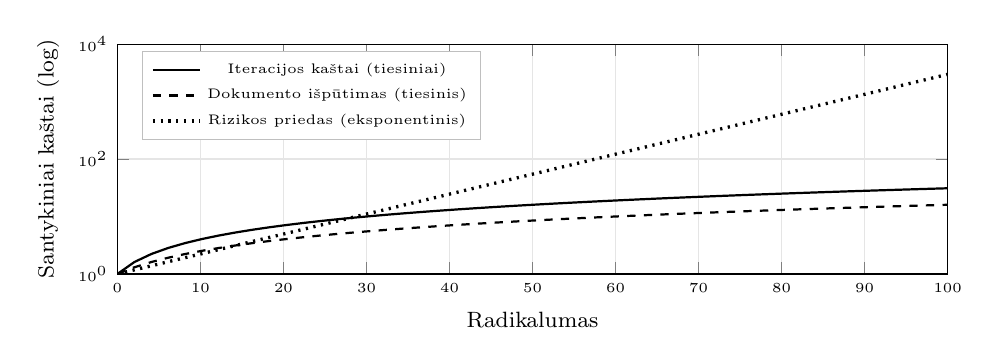
\begin{tikzpicture}
\begin{axis}[
    width=\columnwidth,
    height=4.5cm,
    xlabel={\footnotesize Radikalumas},
    ylabel={\footnotesize Santykiniai kaštai (log)},
    ymode=log,
    xmin=0, xmax=100,
    ymin=1, ymax=10000,
    grid=major,
    grid style={gray!20},
    legend style={at={(0.03,0.97)},anchor=north west,font=\tiny,draw=gray!50},
    tick label style={font=\tiny},
    label style={font=\footnotesize},
]
\addplot[black, thick, domain=0:100, samples=50] {1 + 0.3*x};
\addlegendentry{Iteracijos kaštai (tiesiniai)}
\addplot[black, thick, dashed, domain=0:100, samples=50] {1 + 0.15*x};
\addlegendentry{Dokumento išpūtimas (tiesinis)}
\addplot[black, thick, dotted, line width=1.2pt, domain=0:100, samples=100] {exp(0.08*x)};
\addlegendentry{Rizikos priedas (eksponentinis)}
\end{axis}
\end{tikzpicture}
\caption{Kaštų eskalacija per tris kanalus. Rizikos priedas dominuoja esant dideliam radikalumui.}
\label{fig:radicalism}
\end{figure}

Iš esmės tai nėra cenzūra. Joks teiginys nedraudžiamas. Sistema įkainoja riziką (\ref{tab:costs} lentelė).

\begin{table}[ht]
\centering
\caption{Kaštų palyginimas pagal teiginių tipus.}
\label{tab:costs}
\footnotesize
\begin{tabular}{@{}lcccc@{}}
\toprule
\textbf{Tipas} & \textbf{Iter.} & \textbf{Dok.} & \textbf{Mok.} & \textbf{Iš viso} \\
\midrule
Patikimas & $k_{\min}$ & $B_0$ & $P_{\min}$ & Žemi \\
Ginčytinas & $k_{\text{med}}$ & $B_0{+}k\Delta$ & $\alpha e^{\beta d}$ & Vidutiniai \\
Radikalus & $k_{\max}$ & $\gg B_0$ & $\gg P_{\min}$ & Labai aukšti \\
Apgaulingas & $\to\infty$ & --- & --- & Nepaskelbiamas \\
\bottomrule
\end{tabular}
\end{table}

% ============================================================
% 6. REPUTATION AND RISK
% ============================================================
\section{Reputacija ir rizikos vertinimas}

\subsection{Reputacijos kaupimo modelis}

Reputacija pasižymi trimis savybėmis: \textbf{lėtu kaupimu} (laipsniškas augimas per nuoseklų elgesį), \textbf{greitu sunaikinimu} (viena apgaulė gali katastrofiškai sumažinti balą) ir \textbf{individualiu vertinimu} (kiekviena vartojanti šalis gali taikyti savo apibendrinimo funkciją).

\subsection{Patikimi autoritetai}

Patikimas autoritetas peržiūri teiginius ir, jei įsitikina, kartu pasirašo juos---statydamas savo reputaciją (\ref{fig:authority} pav.). Asimetrija yra numatyta: reputacijos įgijimas yra lėtas (laipsniškas $+\delta$ už kiekvieną sąžiningą patvirtinimą), o jos praradimas yra katastrofiškas ($-\Delta \gg \delta$ už kiekvieną melagingą patvirtinimą; iliustratyviai, pvz., $+2\%$ prieš $-70\%$). Optimali strategija visada yra atmesti įtartinus teiginius. Konkrečios $\delta$ ir $\Delta$ reikšmės yra sistemos parametrai.

\begin{figure}[ht]
\centering
\begin{tikzpicture}[
    box/.style={draw, rounded corners=2pt, minimum width=2cm, minimum height=0.6cm, align=center, font=\scriptsize, fill=black!5},
    arr/.style={-{Stealth[length=4pt]}, thick}
]
\node[box] (exam) at (0,0) {Autoritetas tikrina\\Reputacija: $R$};
\node[box] (true) at (-2,-1.3) {Teisinga: $R{\to}R{+}\delta$\\Daugiau klientų};
\node[box] (false) at (2,-1.3) {Melaginga: $R{\to}R{-}\Delta$\\Klientai palieka};
\node[box] (insight) at (0,-2.6) {Įgijimas: lėtas ($+\delta$)\\Praradimas: staigus ($-\Delta$)};

\draw[arr] (exam) -- node[left,font=\tiny] {tiesa} (true);
\draw[arr] (exam) -- node[right,font=\tiny] {melas} (false);
\draw[arr] (true) -- (insight);
\draw[arr] (false) -- (insight);
\end{tikzpicture}
\caption{Patikimas autoritetas---asimetrinės paskatos.}
\label{fig:authority}
\end{figure}

\subsection{Daugiadimensinė reputacija}

Reputacija yra ne skaliaras, o vektorius per kelias dimensijas: finansinis patikimumas, asmeninis sąžiningumas, profesinė kompetencija, pilietinis įsitraukimas ir kitos (\ref{fig:reputation-radar} pav.). Skirtingi vertinimo teikėjai projektuoja šį vektorių skirtingai, priklausomai nuo konteksto---skolintojas teikia pirmenybę finansiniam patikimumui, darbdavys---profesinei kompetencijai, kaimynas---pilietiniam elgesiui. Nėra vieno „teisingo“ reputacijos balo; tik perspektyvos.

\begin{figure}[ht]
\centering
\begin{tikzpicture}[scale=0.55]
\foreach \a/\l in {90/Finansinis,162/Sąžiningumas,234/Profesinis,306/Pilietinis,18/Socialinis} {
  \draw[gray!40] (0,0) -- (\a:2.5);
  \node[font=\tiny, align=center] at (\a:3.1) {\l};
  \foreach \r in {0.8,1.6,2.4} {
    \fill[black!15] (\a:\r) circle (0.5pt);
  }
}
\draw[thick, fill=black!10] (90:2.0) -- (162:1.2) -- (234:1.8) -- (306:0.9) -- (18:1.5) -- cycle;
\draw[thick, dashed] (90:1.4) -- (162:2.1) -- (234:0.8) -- (306:2.0) -- (18:1.1) -- cycle;
\node[font=\tiny] at (0,-3.3) {Ištisinė: DID A \quad Punktyras: DID B};
\end{tikzpicture}
\caption{Daugiadimensiniai reputacijos vektoriai. Skirtingi DID rodo skirtingus profilius per dimensijas.}
\label{fig:reputation-radar}
\end{figure}

\subsection{Demokratizuotas rizikos vertinimas}

RSN demokratizuoja sisteminį rizikos vertinimą---galimybę, šiuo metu sutelktą finansų institucijose, bet pritaikomą kur kas plačiau nei bankininkystė. Pramoniniai konglomeratai, vertinantys tiekėjų patikimumą, draudimo bendrovės, įkainojančios elgesio riziką, deramas patikrinimas susijungimams ir įsigijimams, įrangos tarnavimo laiko įvertinimas gamyboje---visur, kur sandorio šalies rizika reikalauja vertinimo, RSN teikia decentralizuotą, rinkos vairuojamą alternatyvą. Interpretavimo paslaugų rinka paverčia neapdorotus daugiadimensinius reputacijos duomenis įgyvendinamomis santraukomis, padarydama sandorio šalies vertinimą prieinamą bet kuriam dalyviui ribiniais kaštais.

% ============================================================
% 7. CONSENSUS AND DISPUTE RESOLUTION
% ============================================================
\section{Konsensusas ir ginčų sprendimas}

\subsection{Decentralizuoto teisingumo modelis}

RSN performuluoja teisingumą kaip dvišalio derybų problemą. Nuolatinės, patikrinamos reputacinės žalos grėsmė yra veiksmingesnė atgrasymo priemonė nei teismo procesas, kurio nukentėjusi šalis negali sau leisti.

\subsection{Emergentinis konsensusas}

Kiekvienas dalyvis palaiko asmeninę pasitenkinimo ribą. Tinklo bendras konsensusas atsiranda kaip tūkstančių dvišalių derybų statistinis vidurkis (\ref{fig:consensus} pav.). Atsakas gerokai virš konsensuso (barbariškas) yra brangus paskelbti. Atsakas šalia konsensuso (proporcingas) yra pigus. Konsensusas yra ne taisyklė---jis yra kainos signalas.

\begin{figure}[ht]
\centering
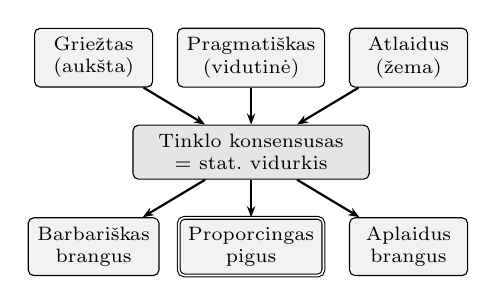
\begin{tikzpicture}[
    person/.style={draw, rounded corners=2pt, minimum width=1.5cm, minimum height=0.5cm, align=center, font=\scriptsize, fill=black!5},
    arr/.style={-{Stealth[length=4pt]}, thick}
]
\node[person] (a) at (-2,0) {Griežtas\\(aukšta)};
\node[person] (b) at (0,0) {Pragmatiškas\\(vidutinė)};
\node[person] (c) at (2,0) {Atlaidus\\(žema)};
\node[person, fill=black!10, minimum width=3cm] (cons) at (0,-1.2) {Tinklo konsensusas\\= stat.\ vidurkis};
\node[person] (exp) at (-2,-2.4) {Barbariškas\\brangus};
\node[person, double] (prop) at (0,-2.4) {Proporcingas\\pigus};
\node[person] (neg) at (2,-2.4) {Aplaidus\\brangus};

\draw[arr] (a) -- (cons);
\draw[arr] (b) -- (cons);
\draw[arr] (c) -- (cons);
\draw[arr] (cons) -- (exp);
\draw[arr] (cons) -- (prop);
\draw[arr] (cons) -- (neg);
\end{tikzpicture}
\caption{Emergentinis konsensusas iš individualių pasitenkinimo ribų.}
\label{fig:consensus}
\end{figure}

\subsection{Bausmės kalibravimas}

Kiekvienas DID turėtojas viešai deklaruoja atsakus į konkrečias netinkamo elgesio kategorijas. Neproporcingai griežtos ar švelnios deklaracijos pritraukia neigiamus reputacijos signalus. Proporcingos deklaracijos priimamos be trinties---savikalibruojanti bausmės sistema.

Konsensuso deklaracijoms taip pat taikoma veidmainystės aptikimas: deklaratyvus įsipareigojimas laikytis konsensuso pozicijos, elgiantis nenuosekliai, yra reputacinis nusižengimas, sunkesnis nei pats nukrypimas, nes rodo tyčinį apgaudinėjimą.

\subsection{Delegavimas}

Visos veiklos DID viduje---su viena išimtimi---gali būti deleguotos kitam DID. \textbf{Subjekto vaidmuo---DID, apie kurio elgesį yra teiginys---negali būti deleguotas; jis yra neperduodamai susietas su tapatybės turėtoju, kuriam teiginys skirtas.} Kiti aktyvūs vaidmenys---Išdavėjas, Autoritetas, Liudytojas, Tikrintojas---gali būti perduoti paskirtam deleguoto DID, ar tai būtų tikrinimui, teiginio pateikimui, dalyvavimui konsensuse ar ginčų sprendimui. Delegavimas gali būti atšauktas bet kuriuo metu. Tai įgalina specializaciją (pvz., profesionalias tikrinimo paslaugas), kol turėtojas išlaiko galutinę kontrolę ir atsakomybę. Delegavimas taikomas visoje sistemoje ir yra būtinas masteliui.

\subsection{Nuo individualios moralės prie emergentinės socialinės sutarties}

Kiekvieno DID deklaruota politika atspindi individualios moralės formalizavimą: ką turėtojas laiko priimtinu, kaip jis reaguoja į konkretų elgesį, ko reikalauja iš sandorio šalių. Šios politikos nėra primetamos sistemos kūrėjo---jas pasirenka kiekvienas dalyvis ir išreiškia mašininiu būdu skaitoma forma.

Šis formalizavimas įgalina trijų etapų emergenciją. Pirma, individuali moralė užkoduojama kaip \textbf{politika}---deklaruotų taisyklių, ribų ir atsako funkcijų rinkinys, kurio DID įsipareigoja laikytis. Antra, visų politikų agregatas visame tinkle sukuria \textbf{emergentinę etiką}---statistiškai stebimas normas, kurių nesukūrė joks vienas dalyvis, bet kurios kyla iš tūkstančių individualių moralinių pozicijų sąveikos~\cite{durkheim1893}. Trečia, ši emergentinė etika, išreikšta kaip bendros elgesio normos, įgyvendinamos per dvišalius kainos signalus, sudaro \textbf{išmatuojamą socialinę sutartį}---ne teorinį konstruktą, kurio niekas nepasirašė~\cite{rawls1971}, o empiriškai stebimą taisyklių rinkinį, paremtą faktiniu elgesiu.

Šis procesas atspindi moralinių pagrindų teorijos išvadas~\cite{haidt2012}: žmogaus moralė yra intuityvi, pliuralistinė ir kultūriškai kintanti. RSN nereikalauja moralinio konsensuso kaip įvesties; jis kuria elgesio konsensusą kaip išvestį. Gauta socialinė sutartis nėra statiška---ji vystosi, kai dalyviai prisijungia, palieka ir koreguoja savo politiką atsakydami į tinklo grįžtamąjį ryšį. Skirtingai nei klasikinė socialinės sutarties teorija, ši sutartis yra atšaukiama, stebima ir įgyvendinama be suvereno.

% ============================================================
% 8. ECONOMIC MODEL
% ============================================================
\section{Ekonominis modelis}

Ankstesniuose skyriuose aprašytas įrankis---RSN tikrinimo mechanizmai, kaštų struktūra ir emergentinis konsensusas. Šis skyrius aprašo metodologiją, kaip taikyti šį įrankį fiskaliniam ir valdymo perėjimui. Įrankis yra universalus; žemiau pateikta metodologija yra viena galima taikymo galimybė.

\subsection{Paskatų struktūra}

Reputacija kaip kapitalas sukuria tiesiogines paskatas sąžiningam elgesiui. Įprastinėje veikloje dalyviai natūraliai kaupia reputaciją per kasdienius sandorius ir įvykdytus įsipareigojimus. Pagrindinės išlaidos tenka \emph{neigiamiems} teiginiams---kitų padarytos žalos fiksavimui. Ši asimetrija skatina naudingą, patikimą elgesį: būti sąžiningam nekainuoja papildomai, o būti žalingam sukuria dokumentuotą pėdsaką, kurį kiti sumokės, kad išsaugotų. Veidmainystė---taisyklių deklaravimas jų nesilaikant---yra brangiausias žlugimo būdas, nes rodo tyčinį apgaudinėjimą.

\subsection{Lygiagreti fiskalinė sistema}

Trys komponentai įgalina konkurencinį spaudimą: (1)~\textbf{Paprastas mokestis}---vienas proporcingas tarifas be išimčių, iš pradžių šiek tiek žemesnis už esamą efektyvųjį tarifą; (2)~\textbf{Elektroninė išlaidų registracija (EIR)}---apverčianti Čekijos EET modelį, kad piliečiai stebėtų valstybės išlaidas; (3)~\textbf{Piliečių valdomas mokesčių paskirstymas}---prasidedantis nuo kelių procentų pirmaisiais metais ir per dešimtmetį pasiekiantis bet kur nuo žemų dviženklių skaičių iki visiškos migracijos prie piliečių valdomos sistemos, priklausomai nuo perėmimo tempo. Faktinis tempas priklauso nuo greičio, kuriuo atsiranda laisvosios rinkos alternatyvos valstybės paslaugoms, ir nuo valstybės noro bendradarbiauti pereinant; laiko funkcija neturi būti tiesinė, ir nėra priežasties nustatyti viršutinę ribą, kur perėmimas galiausiai gali atsirasti.

% ============================================================
% 9. MIGRATION PATH
% ============================================================
\section{Migracijos kelias}

Migracija vyksta per tris etapus (\ref{fig:migration} pav.): \textbf{1 etapas: Perdanga} (RSN kaip informacinis sluoksnis, valstybė yra vienintelis teikėjas), \textbf{2 etapas: Konkurencija} (RSN teikia funkcines alternatyvas, dviejų sistemų naudojimas) ir \textbf{3 etapas: Perėjimas} (RSN lenkia valstybės atitikmenis, savanoriška migracija). Perėjimas yra grįžtamas kiekviename etape.

\begin{figure}[ht]
\centering
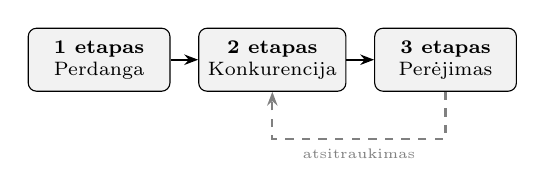
\begin{tikzpicture}[
    phase/.style={draw, rounded corners=3pt, minimum width=1.8cm, minimum height=0.8cm, align=center, font=\scriptsize, fill=black!5},
    arr/.style={-{Stealth[length=5pt]}, thick}
]
\node[phase] (p1) at (0,0) {\textbf{1 etapas}\\Perdanga};
\node[phase] (p2) at (2.2,0) {\textbf{2 etapas}\\Konkurencija};
\node[phase] (p3) at (4.4,0) {\textbf{3 etapas}\\Perėjimas};

\draw[arr] (p1) -- (p2);
\draw[arr] (p2) -- (p3);
\draw[arr, dashed, gray] (p3.south) -- ++(0,-0.6) -| node[below,font=\tiny,pos=0.25] {atsitraukimas} (p2.south);
\end{tikzpicture}
\caption{Trijų etapų migracija---grįžtama kiekviename etape.}
\label{fig:migration}
\end{figure}

Pagrindinis spaudimo mechanizmas yra fiskalinis: kai sąlyginiai mokesčių mokėtojai pasiekia „ekonomiškai reikšmingą mažumą $X$“---grupę, pakankamai didelę, kad represijos prieš ją sukeltų netrivialią ekonominę žalą, o pilietinis nepaklusnumas taptų patikima grėsme---valstybė pradeda derybas. Iliustracijai naudojame $X \approx 15\%$ BVP, bet faktinė riba priklauso nuo konkrečios ekonomikos.

% ============================================================
% 10. SECURITY ANALYSIS
% ============================================================
\section{Saugumo analizė}

Nagrinėjame penkias priešininkų kategorijas: individualius blogus veikėjus, organizuotas grupes, korporacinius priešininkus, valstybinio lygio priešininkus ir protokolo lygio priešininkus.

\textbf{Atsparumas Sybil atakoms}~\cite{douceur2002}. Reputacijos kaupimas reikalauja nuolatinės, patikrinamos sąveikos. Sėkmingos Sybil atakos kaina auga tiesiškai su netikromis tapatybėmis ir kvadratiškai su tiksline reputacijos riba. Kelių DID valdymas lygiagrečiai yra įmanomas, bet brangus pagal projektą---kiekviena tapatybė turi savarankiškai sukaupti reputaciją per tikrą veiklą. Laisvose visuomenėse šie kaštai atgraso nuo atsitiktinio piktnaudžiavimo; diktatūrose lygiagretūs DID tampa išgyvenimo įrankiu, įgalinančiu suskaidytą pasipriešinimą, pogrindinį koordinavimą ir saugesnę juodosios rinkos navigaciją.

\textbf{Apsauga nuo slapto susitarimo.} Abipusio patvirtinimo šablonai tarp uždarų grupių yra aptinkami per socialinio grafo analizę. Reputacijos apibendrinimo funkcijos nuvertina teiginius iš glaudžiai susigrupavusių šaltinių.

\textbf{Valstybinio lygio priešininkas.} Onion maršrutizavimas, centralizuotos infrastruktūros nebuvimas ir Tikrintojo vaidmens paskirstymas visoje dalyvių bazėje užtikrina, kad slopinimas reikalauja priemonių, neproporcingų bet kokiai naudai.

\textbf{Privatumas prieš atskaitomybę.} Pseudonimiškumas---tarpinė padėtis tarp anonimiškumo ir tapatybės atskleidimo---leidžia DID kaupti prasmingą reputaciją neatskleidžiant turėtojo realaus pasaulio tapatybės.

% ============================================================
% 11. PRIVACY
% ============================================================
\section{Privatumo aspektai}

RSN privatumo modelis remiasi pseudonimiškumu. Turėtojas kontroliuoja tapatybės atskleidimą: minimalus (grynas pseudonimas), selektyvus (susieti konkretūs kredencialai) arba pilnas (susieta teisinė tapatybė). Paskelbti teiginiai yra nuolatiniai---sistema palaiko kontekstinį taisymą, bet ne ištrynimą. Turėtojas gali atsisakyti pažeisto DID ir pradėti iš naujo, atsisakydamas sukauptos reputacijos.

% ============================================================
% 12. RELATED WORK
% ============================================================
\section{Susiję darbai}

W3C DID Core specifikacija~\cite{did2022} ir Ceramic Network~\cite{ceramic2023} teikia tapatybės pagrindą. EigenTrust~\cite{kamvar2003} pademonstravo paskirstytą reputacijos apibendrinimą be centrinės institucijos. SBT~\cite{weyl2022} įvedė neperduodamus socialinius žetonus. RSN skiriasi savo dėmesiu ekonominiams kaštams kaip kokybės filtrui ir mechanizmui radikalumui įkainoti.

DAO~\cite{buterin2014} ir kvadratinis balsavimas~\cite{buterin2019} pademonstravo decentralizuoto valdymo įgyvendinamumą. RSN išveda konsensusą iš dvišalių kainos derybų, o ne iš balsavimo.

Pasiūlymas remiasi anarcho-kapitalistine teorija~\cite{rothbard1973,hoppe2001} dėl privataus paslaugų teikimo, bet skiriasi dviem esminiais aspektais: jis projektuoja pyktį ir keršto impulsus, o ne prisiima racionalumą, ir siūlo laipsnišką perėjimą, o ne revoliuciją. Emergentinių socialinių sutarčių koncepcija turi pirmtakų Hayeko spontaniškos tvarkos teorijoje~\cite{hayek1973}.

\textbf{Anarcho-agorizmas.} RSN turi reikšmingų sąlyčio taškų su agoristine kontra-ekonomika~\cite{konkin2006}---ypač akcentu statyti lygiagrečias institucijas ir savanoriškus mainus. Tačiau agorizmas linkęs prisiimti racionalų savanaudiškumą kaip pakankamą koordinavimo mechanizmą ir dažnai stokoja konkretaus migracijos kelio nuo esamų valstybės struktūrų. RSN aiškiai įtraukia neracionalius elgesio polinkius ir teikia fiskalinį spaudimo mechanizmą laipsniškam perėjimui.

\textbf{Meritokratija.} RSN gali atspindėti pirmąjį funkcinį aprašymą, kaip meritokratija~\cite{young1958} gali atsirasti kaip sisteminė savybė, o ne šūkis. Tradicinės meritokratinės sistemos žlunga, nes reikalauja centrinės institucijos „nuopelnams“ apibrėžti ir įgyvendinti. RSN nuopelnai atsiranda iš dvišalių vertinimų: tie, kurie teikia vertę, kaupia reputaciją; joks komitetas nesprendžia, kas turi nuopelnų.

\textbf{Nuosavybė kaip privilegija.} RSN iš esmės skiriasi nuo anarcho-kapitalistinio ir Austrijos mokyklos nuosavybės teisių kaip natūralių ir absoliučių traktavimo. RSN sistemoje nuosavybė yra \emph{privilegija}---socialinis pripažinimas, kuris kraštutiniais atvejais gali būti atimtas bendruomenės, kai dalyvis iš esmės pažeidžia bendras normas (išdavystė, atsisakymas ginti bendruomenę egzistencinės krizės metu, sisteminis išnaudojimas). Tai nėra valstybės nusavinimas, o socialinio pripažinimo atėmimas dvišalių santykių tinklo.

% ============================================================
% 13. LIMITATIONS
% ============================================================
\section{Diskusija ir apribojimai}

\textbf{Šaltas startas.} RSN vertė priklauso nuo tinklo efektų; ankstyvieji perėmėjai susiduria su ribota verte, kol dalyvavimas nepasiekia ribos. Tačiau net nuo ankstyvųjų etapų DID tinklas tarnauja kaip naudingas papildomas informacijos šaltinis. Tikimasi, kad ankstyvasis reputacijos vertinimas ir autoriteto įvertinimas vystysis palaipsniui, didėjant sudėtingumui.

\textbf{Apsauga nuo išnaudojimo ir prieigos kontrolė.} Tiksliniai DID gali nustatyti laipsniškus mokesčius ir prieigos apribojimus užklausoms iš žemos reputacijos DID. Tai nėra dvejetainis, o tolydi skalė: kuo mažiau reputacijos turi užklausiantis DID, tuo mažiau informacijos jis gauna, tuo ilgiau laukia ir tuo daugiau moka. Šis mechanizmas skatina tikrą dalyvavimą, o ne pasyvų vartojimą.

\textbf{Prieigos nelygybė.} Teiginių skelbimo kaina gali atfiltruoti teisėtus nusiskundimus iš ekonomiškai nepalankioje padėtyje esančių dalyvių. Sušvelninimas: kiekvienas dalyvis vienu metu tarnauja kaip potencialus tikrintojas (arba deleguoja šį vaidmenį) ir uždirba tikrinimo mokesčius. Per pakankamą laiko horizontą neradikalus dalyvis turėtų priartėti prie finansinio neutralumo---tikrinimo pajamos maždaug kompensuoja skelbimo kaštus. Tai statistinis lūkestis, o ne garantija.

\textbf{Reputacijos nelygybė.} Ankstyvieji perėmėjai kaupia pranašumus, kurie gali sukurti kliūtis vėlyviesiems. Tačiau reputacijos vertinimą atlieka trečiųjų šalių teikėjai, kurie gali pasirinkti sušvelninti pirmtako pranašumą per savo apibendrinimo algoritmus. Būti pirmam su gera reputacija yra teisėtas lyginamasis ekonominis pranašumas---ir tai yra pagal projektą.

\textbf{Atviri klausimai.} Optimalios kaštų funkcijos, apibendrinimo standartai, protokolo valdymas ir sąveika su DI sugeneruotais sintetiniais reputacijos duomenimis lieka būsimo darbo sritimis.

Šis straipsnis neteigia, kad RSN sukurs optimalius rezultatus visomis aplinkybėmis. Jis teigia, kad RSN atspindi \emph{įgyvendinamą} alternatyvą---techniškai realizuojamą, ekonomiškai save išlaikančią ir socialiai suderinamą su žmogaus elgesio polinkiais tokiais, kokie jie iš tikrųjų yra.

% ============================================================
% 14. CONCLUSION
% ============================================================
\section{Išvados}

Šiame straipsnyje pristatytas reputacijos socialinis tinklas---decentralizuotas protokolas, įgalinantis pseudonimišką, patikrinamą reputacijos mainai. Brangaus radikalumo principas užtikrina, kad apgaulingi teiginiai būtų įkainojami už ribų be cenzūros. Siūlomas migracijos kelias įgalina laipsnišką, grįžtamą perėjimą nuo esamų institucijų. Projektas įtraukia žmogaus prigimtį tokią, kokia ji yra---įskaitant smulkmeniškumą, pyktį ir keršto pasitenkinimo troškimą---o ne reikalauja ideologinės transformacijos. Rezultatas yra ne utopija, o sistema, kurioje teisingumas yra prieinamas, reputacija yra užsitarnaujama, o netinkamo elgesio kaina tenka tai šaliai, kuri jį sukėlė.

% ============================================================
% REFERENCES
% ============================================================
\bibliography{references}

\end{document}
